\subsection{Server}

The server is a stateful one, which means that mantain information on the
connection. It is composed by a \code{ThreadPool} which handles the requests
from the clients and processes them. The connection persists until the client's
logout. After that a connection is established a thread will handle the requests
coming from that connection, it will parse that request and issue the correct
query to the database, via JPA\@. After the query is performed the result will
be sent back to the client. The diagram in Figure~\ref{fig:server} shows the
implementation of the server's classes.

\begin{landscape}
	\begin{figure}
		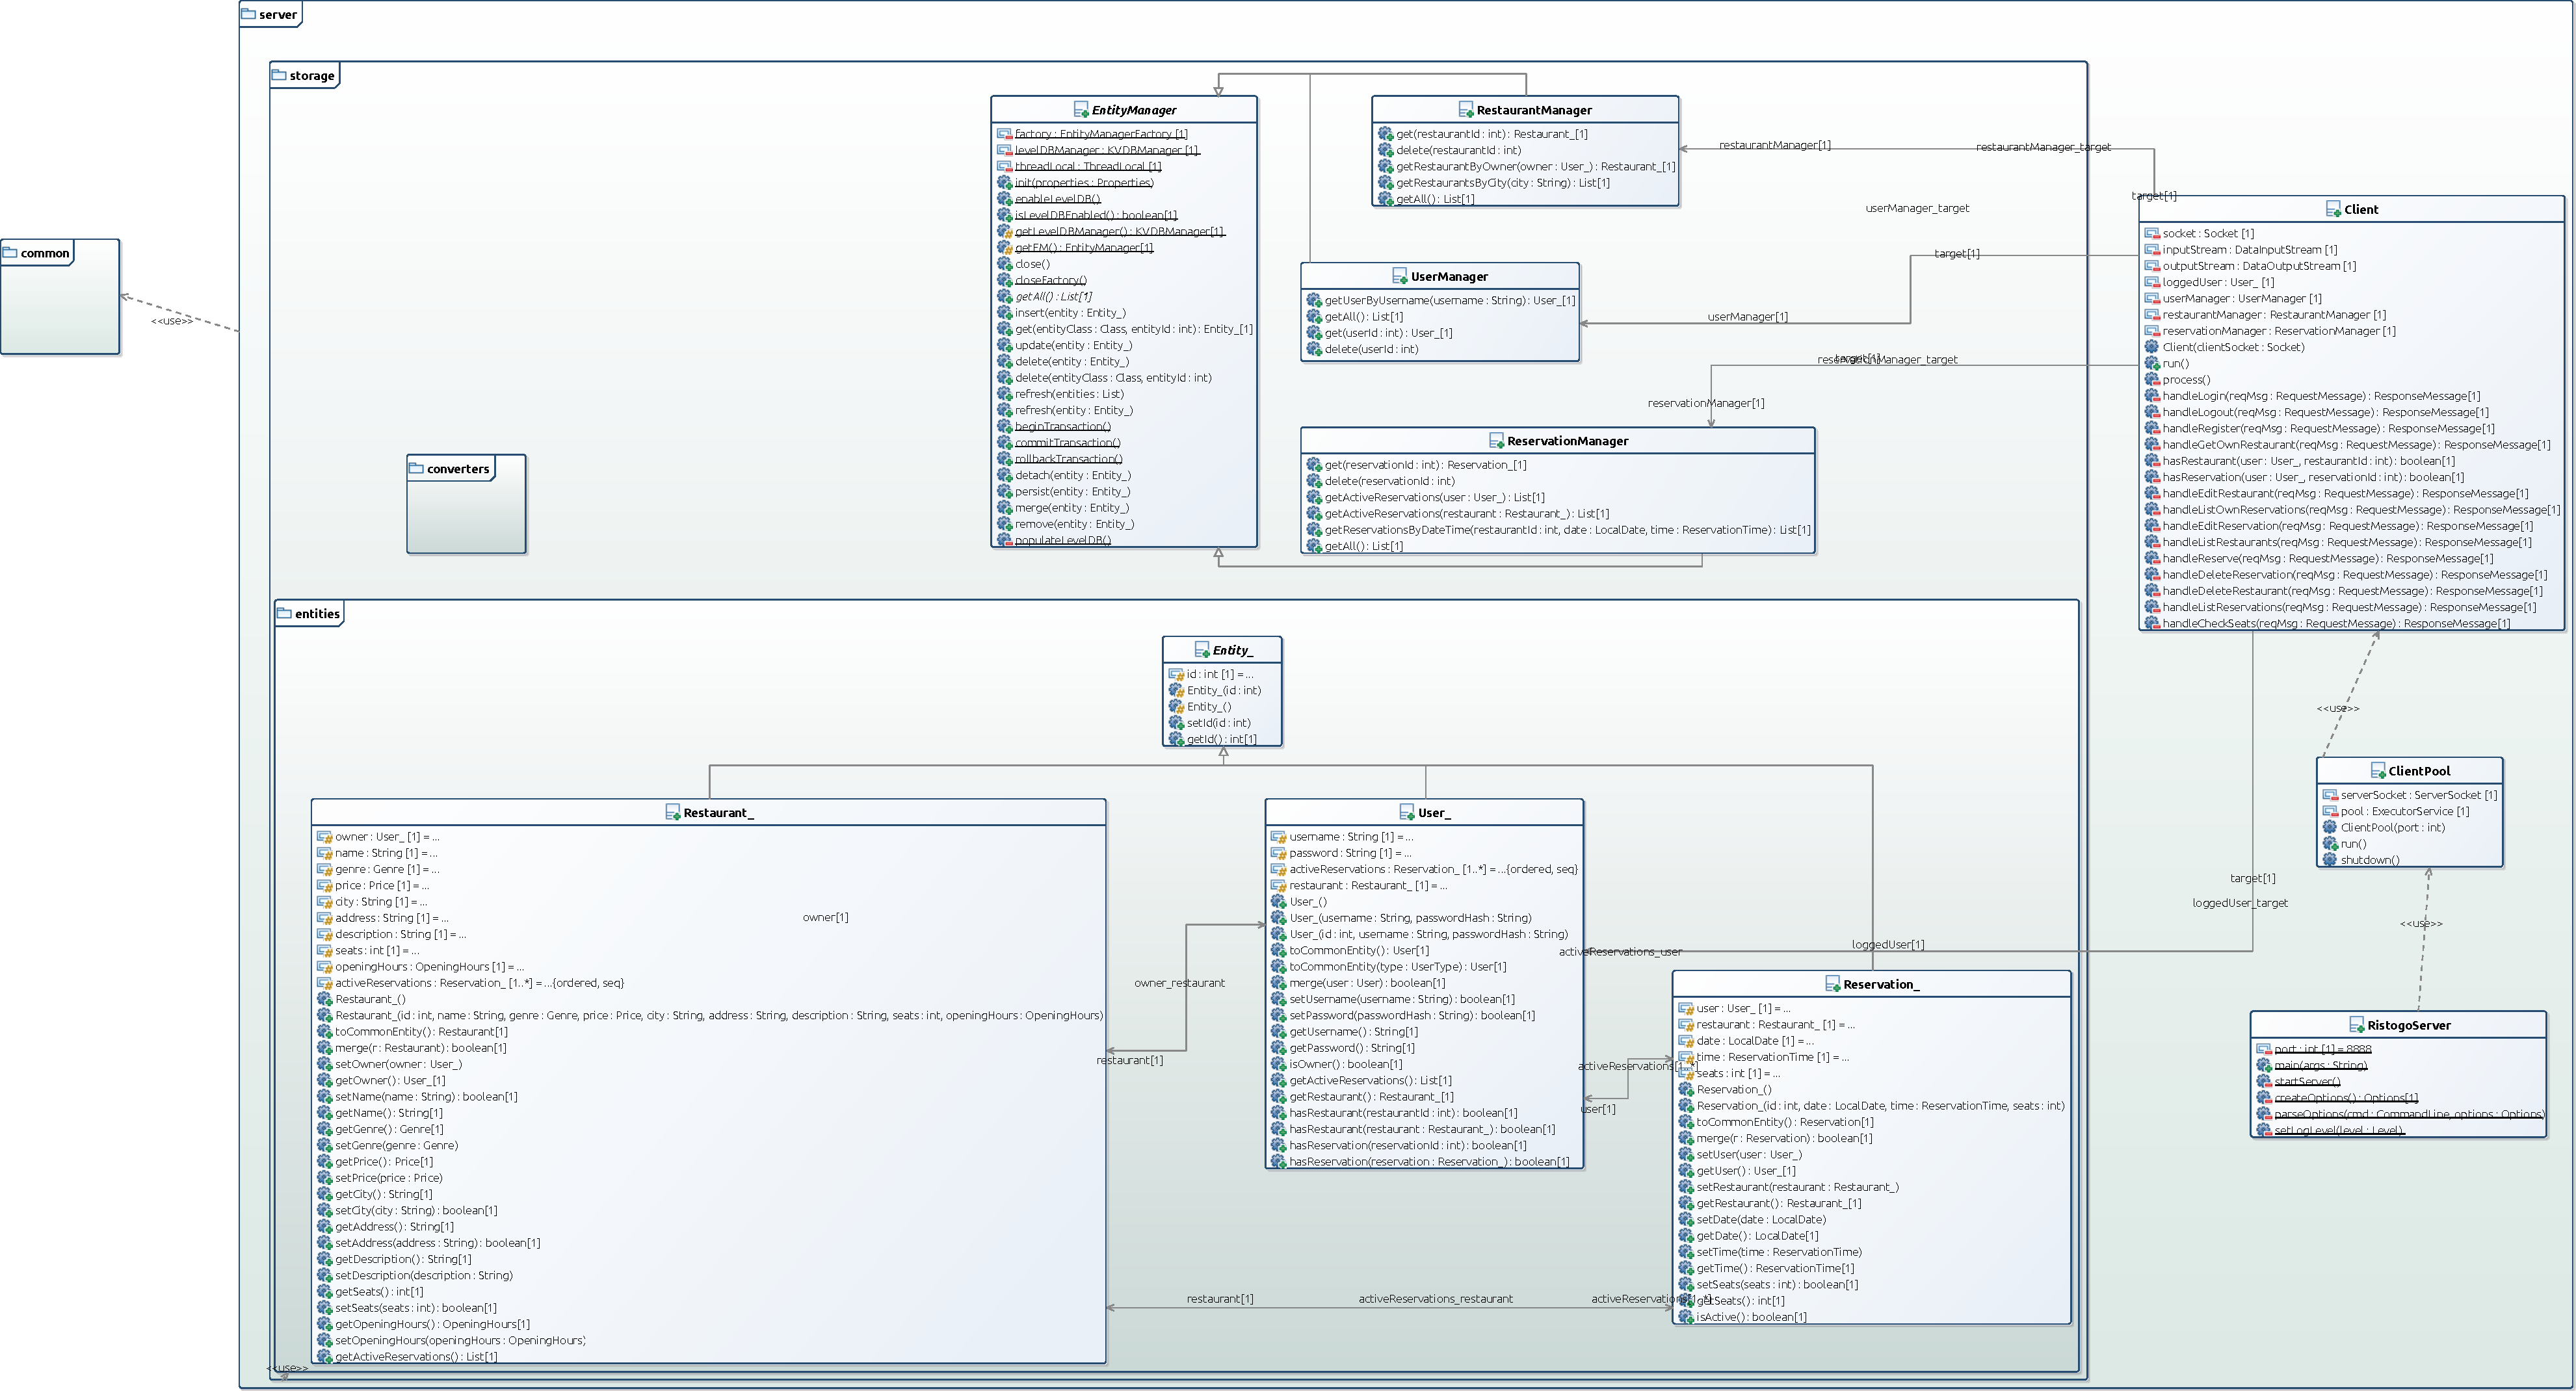
\includegraphics[width=0.85\paperheight]{server}
		\caption{\code{ristogo.server} UML Implementation Diagram.}
		\label{fig:server}
	\end{figure}
\end{landscape}
